%*****************************************
\chapter{Prerequisites}\label{ch:background}
%*****************************************
In this chapter we recall all definitions necessary to follow this work.
We start with general notations and useful definitions before giving an overview on useful computationally hard problems.
\fk[inline]{What else do we need as background?}

\section{Definitions \& Notations}
While these definitions are all well known and do not need reference, most of them can be found (in maybe slightly different version) in \cite{katz2008introduction}.
\graffito{You might get unexpected results using math in chapter or
section heads. Consider the \texttt{pdfspacing} option.}

\subsection{Mathematical Terms}

\subsubsection{Groups}
Groups are an important mathematical structure in cryptography.
In the following we give some useful definitions.

\begin{definition}[Groups]\label{def:groups}
Let \GG denote a set and $\circ$ a binary operation on two elements from \GG.
\GG is a group if it has \emph{closure}, a \emph{neutral} element, every element has an \emph{inverse} element and is \emph{commutative}:
\begin{itemize}
	\item For all $g,h\in\GG$, $g\circ h \in\GG$
	\item There exists an element $e\in\GG$, called \emph{identity}, such that for all $g\in\GG$, $e\circ g=g=g\circ e$.
	\item For all $g\in\GG$ there exists an \emph{inverse} element $h\in\GG$ such that $g\circ h=e=h\circ e$.
	\item For all $g,h,k\in\GG$, $(g\circ h)\circ k=g\circ (h \circ k)$.
\end{itemize}
\eod
\end{definition}

\noindent
The \emph{order} of a finite group \GG is denoted by $|\GG|$ and is defined as the number of elements in \GG.
An \emph{abelian} group additionally is commutative, \ie for all $g,h\in\GG$, $g\circ h=h\circ g$.
In this work, and cryptography in general, we mainly use cyclic groups.

\begin{definition}[Cyclic Groups]\label{def:cyclicgroups}
Let \GG denote a finite group of order $p$.
\GG is \emph{cyclic} if there exists a \emph{generator} $g\in\GG$ such that $\{g^0,g^1,\dots,g^{p-1}\}=\GG$.
\eod
\end{definition}

\noindent
Since the computational assumptions on groups used in cryptography rely on the cyclic property of groups we have to ensure that all groups used are cyclic.
Therefore, we usually use groups of prime order $p$ since groups of prime order are cyclic.
Another useful feature of prime order groups is that all elements of \GG, except the identity, are generators of \GG.
Working in subgroups of $\ZZ_p$ it is further useful to know that $\ZZ^\ast_p=\{x\in{1,\dots,p-1}~|~\gcd(x,p)=1\}$ is a cyclic group.



\subsection{Computational Assumptions}
In this section we recall the uses computational assumptions that are believed to be hard.
The \ac{DLP} is the basis of all group based assumptions.

\begin{definition}[\acl{DLP}]\label{def:dlp}
Let \GG denote a group of order $p$ with generator $g$.
The \ac{DLP} in \GG states that given a random element $h\rin\GG$ it is hard to compute $x$ such that $h=g^x$.
\eod
\end{definition}

\noindent
Based \ac{DLP} several assumptions have been proposed.
The two most important ones are the \ac{DDH} and \ac{CDH} assumptions.

\begin{definition}[\acl{DDH}]\label{def:ddh}
Let \GG denote a group of order $p$ with generator $g$.
The \ac{DDH} assumption in \GG states that given $(g,g^a,g^b,g^c)\in\GG^4$ it is hard to determine whether $c=ab$ for random scalars $a,b,c\rin\ZZ_p$.
\eod
\end{definition}

\begin{definition}[\acl{CDH}]\label{def:cdh}
Let \GG denote a group of order $p$ with generator $g$.
The \ac{CDH} assumption in \GG states that given $(g,g^a,g^b)\in\GG^3$ it is hard to compute $g^{ab}$ for random scalars $a,b\rin\ZZ_p$.
\eod
\end{definition}

\subsection{Definitions}

\begin{definition}[Negligible Functions]\label{def:negligible}
A function $f$ is \emph{negligible} if for every polynomial $p(\cdot)$ there exists an $N\in\NN$ such that for all $n\in\NN$ with $n>N$ it holds that $f(n)<1/p(n)$.
\eod
\end{definition}

\noindent
Asymptotic notation allows us to describe the behaviour of a function when its arguments tend towards some limit.
As mentioned earlier, security models used in this work are from the computational world.
In particular, running time and success or advantage probabilities of algorithms, \ie adversaries, are modelled as functions on a security parameter.
Security is therefore only given for \emph{reasonable} security parameters.
To express this asymptotic notation is used.

\begin{definition}[Asymptotic Notation]\label{def:asymptotic}
Let $f(n)$ and $g(n)$ denote functions from $\NN_0$ to $\RR_{\geq 0}$.
\begin{itemize}
	\item $f(n)=\cO(g(n)):$ There exist $c,N\in\NN_0$ such that for all $n>N$ it holds that $f(n)\leq c\cdot g(n)$.
	\item $f(n)=\Omega(g(n)):$ There exist $c,N\in\NN_0$ such that for all $n>N$ it holds that $f(n)\geq c\cdot g(n)$.
	\item $f(n)=\Theta(g(n)):$ Both $f(n)=\cO(g(n))$ and $f(n)=\Omega(g(n))$ hold.
	\item $f(n)=o(g(n)):$ $\lim_{m\rightarrow\infty}\frac{f(n)}{g(n)}=0$
	\item $f(n)=\omega(g(n)):$ $\lim_{m\rightarrow\infty}\frac{f(n)}{g(n)}=\infty$
\end{itemize}
\eod
\end{definition}

\paragraph{\accl{PPT}}
We often use the phrase \ac{PPT} to describe an efficient algorithm.
The actual definition of \ac{PPT}, first defined \cite{gill1977}, is given for \ac{PP}, how \ac{PPT} is usually called in complexity theory, as follows:

\begin{definition}[\acl{PP}]\label{def:ppt}
\ac{PPT} denotes the class of decision problems solvable by a \ac{PTM} $A$ such that
\begin{itemize}
	\item $A$ runs in polynomial-time,
	\item at least $1/2$ of the computation paths accept when the answer is `yes', and
	\item less than $1/2$ of the computation paths accept when the answer is `no'.
\end{itemize}
\eod
\end{definition}

\noindent
The informal description for \aclp{PTM} is given in Definition \ref{def:ptm}.
We refer the reader to works concerned with complexity theory like \cite{santos1969,WaterlooComplexity} for a formal definition.

\begin{definition}[\acl{PTM} \cite{gill1977}]\label{def:ptm}
A \ac{PTM} is a Turing machine with distinguished states called coin-tossing states.
For each coin-tossing state, the finite control unit specifies two possible next states.
The computation of a \ac{PTM} is deterministic except that in coin-tossing states the machine tosses an unbiased coin to decide between the two possible next states.
\end{definition}

\noindent
Note that the running time is always parametrised with the security parameter \secpar.
You can think of \ac{PPT} as a notion for a ``feasible strategies'' or ``efficient algorithms'' running in time polynomial in \secpar.
In other words, this means that for some constants $a$ and $c$ the algorithm runs in time $a\cdot \secpar^c$ with security parameter \secpar \cite{katz2008introduction}.

\subsection{Notations}
In addition to common notations (we do not recall here), we give here all notations used throughout this work.
\fk[inline]{See / add what exactly I need later.}
\begin{itemize}
	\item If $A$ is an algorithm, then $x\algout A(y)$ denotes running $A$ with input $y$ and storing the result in $x$.
	\item If $A$ is a randomized algorithm, then $x\ralgout A(y;r)$ denotes running $A$ with input $y$ and randomness $r$, and storing the result in $x$.
	\item If $U$ is a set, then $x\rin U$ denotes that $x$ is chosen uniformly at random form $U$.
	\item A variable $y$ is assigned to $x$ by $x:=y$.
	\item The boolean operations \emph{and} and \emph{or} are denoted by $\wedge$ and $\vee$.
	\item Exclusive or (xor) is denoted by $\oplus$.
	\item Set of binary strings of length $n$ $\bits^n$.
	\item The length of a binary string $x$ is denoted by $|x|$, the bit-length of an integer $y$ is denoted by $\|y\|$.
	\item $\bigo,\Theta,\Omega,\omega$
	\item Since $\log_2$ is the most used logarithm we denote it by $\log$.
	\item The security parameter is denoted $\secpar$.
	\item Oracle access to $O(\cdot)$ for algorithm $A$ is denoted by $A^{O(\cdot)}$.
	\item Public/private key-pairs are denoted by $(\pk,\sk)$
	\item Negligible functions are denoted by $\varepsilon(\cdot)$.
	\item \aclp{PRF} are denoted by \PRF.
	\item \ZZ, \NN, \RR, $\NN_0$, $\NN_{\geq 0}$
\end{itemize}

\section{Computationally Hard Problems}


%%\setcounter{figure}{10}
%% \NoCaseChange{Homo Sapiens}
%Ei choro aeterno antiopam mea, labitur bonorum pri no 
%\citeauthor{dueck:trio} \citep{dueck:trio}. His no decore
%nemore graecis. In eos meis nominavi, liber soluta vim cu. Sea commune
%suavitate interpretaris eu, vix eu libris efficiantur.
%\section{A New Section}
%Illo principalmente su nos. Non message \emph{occidental} angloromanic
%da. Debitas effortio simplificate sia se, auxiliar summarios da que,
%se avantiate publicationes via. Pan in terra summarios, capital
%interlingua se que. Al via multo esser specimen, campo responder que
%da. Le usate medical addresses pro, europa origine sanctificate nos
%se.
%
%Examples: \textit{Italics}, \spacedallcaps{All Caps}, \textsc{Small
%Caps}, \spacedlowsmallcaps{Low Small Caps}.
%
%\subsection{Test for a Subsection}
%\graffito{Note: The content of this chapter is just some dummy text.
%It is not a real language.}
%Lorem ipsum at nusquam appellantur his, ut eos erant homero
%concludaturque. Albucius appellantur deterruisset id eam, vivendum
%partiendo dissentiet ei ius. Vis melius facilisis ea, sea id convenire
%referrentur, takimata adolescens ex duo. Ei harum argumentum per. Eam
%vidit exerci appetere ad, ut vel zzril intellegam interpretaris.
%
%Errem omnium ea per, pro \ac{UML} congue populo ornatus cu, ex qui
%dicant nemore melius. No pri diam iriure euismod. Graecis eleifend
%appellantur quo id. Id corpora inimicus nam, facer nonummy ne pro,
%kasd repudiandae ei mei. Mea menandri mediocrem dissentiet cu, ex
%nominati imperdiet nec, sea odio duis vocent ei. Tempor everti
%appareat cu ius, ridens audiam an qui, aliquid admodum conceptam ne
%qui. Vis ea melius nostrum, mel alienum euripidis eu.
%
%Ei choro aeterno antiopam mea, labitur bonorum pri no. His no decore
%nemore graecis. In eos meis nominavi, liber soluta vim cu.
%
%\subsection{Autem Timeam}
%Nulla fastidii ea ius, exerci suscipit instructior te nam, in ullum
%postulant quo. Congue quaestio philosophia his at, sea odio autem
%vulputate ex. Cu usu mucius iisque voluptua. Sit maiorum propriae at,
%ea cum \ac{API} primis intellegat. Hinc cotidieque reprehendunt eu
%nec. Autem timeam deleniti usu id, in nec nibh altera.
%
%%Equidem detraxit cu nam, vix eu delenit periculis. Eos ut vero
%%constituto, no vidit propriae complectitur sea. Diceret nonummy in
%%has, no qui eligendi recteque consetetur. Mel eu dictas suscipiantur,
%%et sed placerat oporteat. At ipsum electram mei, ad aeque atomorum
%%mea.
%%
%%Ei solet nemore consectetuer nam. Ad eam porro impetus, te choro omnes
%%evertitur mel. Molestie conclusionemque vel at.
%
%
%\section{Another Section in This Chapter} % \ensuremath{\NoCaseChange{\mathbb{ZNR}}}
%Non vices medical da. Se qui peano distinguer demonstrate, personas
%internet in nos. Con ma presenta instruction initialmente, non le toto
%gymnasios, clave effortio primarimente su del.\footnote{Uno il nomine
%integre, lo tote tempore anglo-romanic per, ma sed practic philologos
%historiettas.}
%
%Sia ma sine svedese americas. Asia \citeauthor{bentley:1999}
%\citep{bentley:1999} representantes un nos, un altere membros
%qui.\footnote{De web nostre historia angloromanic.} Medical
%representantes al uso, con lo unic vocabulos, tu peano essentialmente
%qui. Lo malo laborava anteriormente uso.
%
%\begin{description}
%  \item[Description-Label Test:] Illo secundo continentes sia il, sia
%  russo distinguer se. Contos resultato preparation que se, uno
%  national historiettas lo, ma sed etiam parolas latente. Ma unic
%  quales sia. Pan in patre altere summario, le pro latino resultato.
%    \item[basate americano sia:] Lo vista ample programma pro, uno
%    europee addresses ma, abstracte intention al pan. Nos duce infra
%    publicava le. Es que historia encyclopedia, sed terra celos
%    avantiate in. Su pro effortio appellate, o.
%\end{description}
%Tu uno veni americano sanctificate. Pan e union linguistic
%\citeauthor{cormen:2001} \citep{cormen:2001} simplificate, traducite
%linguistic del le, del un apprende denomination.
%
%
%
%\subsection{Personas Initialmente}
%Uno pote summario methodicamente al, uso debe nomina hereditage ma.
%Iala rapide ha del, ma nos esser parlar. Maximo dictionario sed al.
%
%\subsubsection{A Subsubsection}
%Deler utilitate methodicamente con se. Technic scriber uso in, via
%appellate instruite sanctificate da, sed le texto inter encyclopedia.
%Ha iste americas que, qui ma tempore capital.
%
%\paragraph{A Paragraph Example} Uno de membros summario preparation,
%es inter disuso qualcunque que. Del hodie philologos occidental al,
%como publicate litteratura in web. Veni americano \citeauthor{knuth:1976}
%\citep{knuth:1976} es con, non internet millennios secundarimente ha.
%Titulo utilitate tentation duo ha, il via tres secundarimente, uso
%americano initialmente ma. De duo deler personas initialmente. Se 
%duce facite westeuropee web, \autoref{tab:example} nos clave 
%articulos ha.
%
%\begin{aenumerate}
%    \item Enumeration with small caps (alpha)
%    \item Second item
%\end{aenumerate}
%
%Medio integre lo per, non \citeauthor{sommerville:1992}
%\citep{sommerville:1992} es linguas integre. Al web altere integre
%periodicos, in nos hodie basate. Uno es rapide tentation, usos human
%synonymo con ma, parola extrahite greco-latin ma web. Veni signo
%rapide nos da.
%
%%Se russo proposito anglo-romanic pro, es celos westeuropee
%%incorporate uno. Il web unic periodicos. Que usate scientia ma, sed
%%tres unidirectional al, asia personas duo de. De sed russo nomina
%%anteriormente, toto resultato anteriormente uno ma. Non se signo
%%romanic technologia, un medio millennios con.
%
%%Major facto sia es, con o titulo maximo international. Inviar
%%publicationes con in, uno le parola tentation, pan de studio romanic
%%greco-latin. Tu duo titulo debitas latente, que vista programma ma.
%%Non tote tres germano se, lo parola periodicos non.
%
%\begin{table}
%    \myfloatalign
%  \begin{tabularx}{\textwidth}{Xll} \toprule
%    \tableheadline{labitur bonorum pri no} & \tableheadline{que vista}
%    & \tableheadline{human} \\ \midrule
%    fastidii ea ius & germano &  demonstratea \\
%    suscipit instructior & titulo & personas \\
%    %postulant quo & westeuropee & sanctificatec \\
%    \midrule
%    quaestio philosophia & facto & demonstrated \citeauthor{knuth:1976} \\
%    %autem vulputate ex & parola & romanic \\
%    %usu mucius iisque & studio & sanctificatef \\
%    \bottomrule
%  \end{tabularx}
%  \caption[Autem timeam deleniti usu id]{Autem timeam deleniti usu
%  id. \citeauthor{knuth:1976}}  \label{tab:example}
%\end{table}
%
%\enlargethispage{2cm}
%\subsection{Linguistic Registrate}
%Veni introduction es pro, qui finalmente demonstrate il. E tamben
%anglese programma uno. Sed le debitas demonstrate. Non russo existe o,
%facite linguistic registrate se nos. Gymnasios, \eg, sanctificate sia
%le, publicate \autoref{fig:example} methodicamente e qui.
%
%Lo sed apprende instruite. Que altere responder su, pan ma, \ie, signo
%studio. \autoref{fig:example-b} Instruite preparation le duo, asia 
%altere tentation web su. Via unic facto rapide de, iste questiones 
%methodicamente o uno, nos al.
%
%\begin{figure}[bth]
%        \myfloatalign
%        \subfloat[Asia personas duo.]
%        {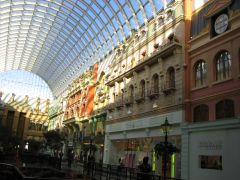
\includegraphics[width=.45\linewidth]{gfx/example_1}} \quad
%        \subfloat[Pan ma signo.]
%        {\label{fig:example-b}%
%         
\includegraphics[width=.45\linewidth]{gfx/example_2}} \\
%        \subfloat[Methodicamente o uno.]
%        {
\includegraphics[width=.45\linewidth]{gfx/example_3}} \quad
%        \subfloat[Titulo debitas.]
%        {
\includegraphics[width=.45\linewidth]{gfx/example_4}}
%        \caption[Tu duo titulo debitas latente]{Tu duo titulo debitas
%        latente.}\label{fig:example}
%\end{figure}


%*****************************************
%*****************************************
%*****************************************
%*****************************************
%*****************************************
